\documentclass[a4paper]{article}
\usepackage[margin=1in]{geometry}
\usepackage[table]{xcolor}
\usepackage{graphicx}
\usepackage{caption}
\graphicspath{ {images/} }   



\begin{document}
\author{Bence Mih\'aly K\'otis}
\title{Quantophile: Trading Framework Design Document}
\maketitle

\clearpage

\tableofcontents

\clearpage
\section{Abstract }
This document describes the basic design of the Quantophile trading framework. 


%%%%%%%%%%%%%%%%%%%%%%%%%%%%%%%%%%%%%%%%%%%%%%%%%%%%%%%%%%%%%%%%%%%%%%%%%%%%%%%    
\section{Overview}
    Quantophile is a trading framework written in C++, with a web interface. The term "Trading Framework" refers to the fact that quantophile was made to be customizable. It implements features such as crawling trading data, then cleaning it up, to be save in a database. This becomes useful if one wants to accumulate second resolution data for free. Quantophile takes in a python script as a trading strategy.


    
   \begin{center}
    \begin{figure}[h]
    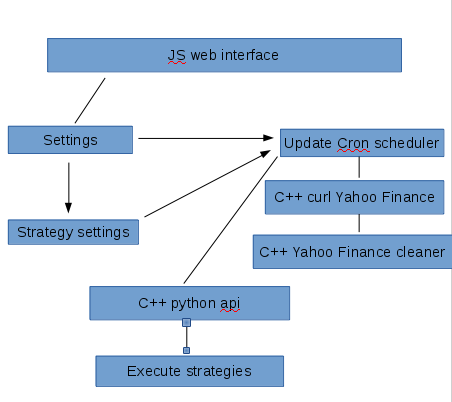
\includegraphics[height=10cm, width=10cm] {overview.png}
    \caption{Overview}
    \end{figure}
    \end{center}



\section{Interface customization}
    Quantophile will keep a live graph on the dashboard of any variable that you wish. You can specify which variable you want to print, using the API. You can also enable built in functions such as budget tracking, etc.

\section{Data acquisition}
    At the moment, Quantophile only supports pulling and cleaning data from yahoo finance. 

\section{Python strategies}
    Quantophile supports all quantitative python functions, since it is essentially a wrapper with some bells and whistles that gets data from the user's phython script.
           



\end{document}
